\documentclass{article}

% if you need to pass options to natbib, use, e.g.:
%     \PassOptionsToPackage{numbers, compress}{natbib}
% before loading neurips_2023

% ready for submission
\usepackage[final]{neurips_2023}

% to avoid loading the natbib package, add option nonatbib:
%    \usepackage[nonatbib]{neurips_2023}


\usepackage[utf8]{inputenc} % allow utf-8 input
\usepackage[T1]{fontenc}    % use 8-bit T1 fonts
\usepackage{hyperref}       % hyperlinks
\usepackage{url}            % simple URL typesetting
\usepackage{booktabs}       % professional-quality tables
\usepackage{amsfonts}       % blackboard math symbols
\usepackage{nicefrac}       % compact symbols for 1/2, etc.
\usepackage{microtype}      % microtypography
\usepackage{xcolor}         % colors

\usepackage{enumitem}
\usepackage{graphicx}
\usepackage[font=small,skip=2pt]{caption}
\usepackage{lipsum}         % placeholder text generation
\usepackage{subcaption} 


% Damit die (sub)sections wie in der angabe formatiert sind: 1.), ..., a.), ...
\renewcommand{\thesection}{\arabic{section}.)}
\renewcommand{\thesubsection}{\alph{subsection}.)}


\title{MLPC Report  - Task 3: Classification Experiments}


% The \author macro works with any number of authors. There are two commands
% used to separate the names and addresses of multiple authors: \And and \AND.
%
% Using \And between authors leaves it to LaTeX to determine where to break the
% lines. Using \AND forces a line break at that point. So, if LaTeX puts 3 of 4
% authors names on the first line, and the last on the second line, try using
% \AND instead of \And before the third author name.


% Sorry, musste die Namen alphabetisch anordnen, hätte mich sonst zu sehr getriggered :(
% Kein Problem die Anordnung war wie die Gruppen Liste im Moodle ist.

\author{
  Team OBSERVE \AND
  Johannes Grafinger 
  \And
  Jonas Gantar 
  \And 
  Leonhard Markus Spanring 
  \And 
  Reinhard Josef Pötscher
}

\begin{document}

\maketitle

\begin{contributions}
  \textcolor{blue}{As a group a solution approach was discussed for each question, then the questions were answered by individuals or sub-groups.} 
  \textcolor{magenta}{Task 1 was completed by Jonas and Johannes. Task 2 was implemented by Johannes and answered by Reinhard. Task 3 was attempted by Jonas, Johannes and Reinhard independently and then answered by Johannes as he produced the best results. Task 4 was answered be Reinhard. Task 5 was discussed as a group and completed by Leo (including training the classifiers). Task 6 was completed by Johannes and Leo.} 
  \textcolor{green}{Collaboration was done over GitHub and project progression was tracked through regular stand-ups.} 
\end{contributions}


\section{Labeling Function}
\label{sec:Labeling Function}



For your analysis, you may focus on a subset of the 58 classes provided.



\subsection{Assess how accurately the applied labeling functions capture the intended classes. }
\label{sec:Labeling Function:a}



\subsubsection{Do the mapped classes correspond well to the free-text annotations? }
\label{sec:Labeling Function:a-1}



\subsubsection{Are the labeled events clearly audible within the indicated time regions? }
\label{sec:Labeling Function:a-2}






\subsection{Which audio features appear most useful for distinguishing between the classes of interest? }
\label{sec:Labeling Function:b}






\subsection{How well do the chosen audio features group according to the discretized class labels? }
\label{sec:Labeling Function:c}



\subsubsection{Do samples of the same class form tight clusters? }
\label{sec:Labeling Function:c-1}




%\newpage


\section{Data Split} 
\label{sec:Data Split}


\begin{figure}[htbp]
  \centering
  \begin{subfigure}[b]{0.49\textwidth}
    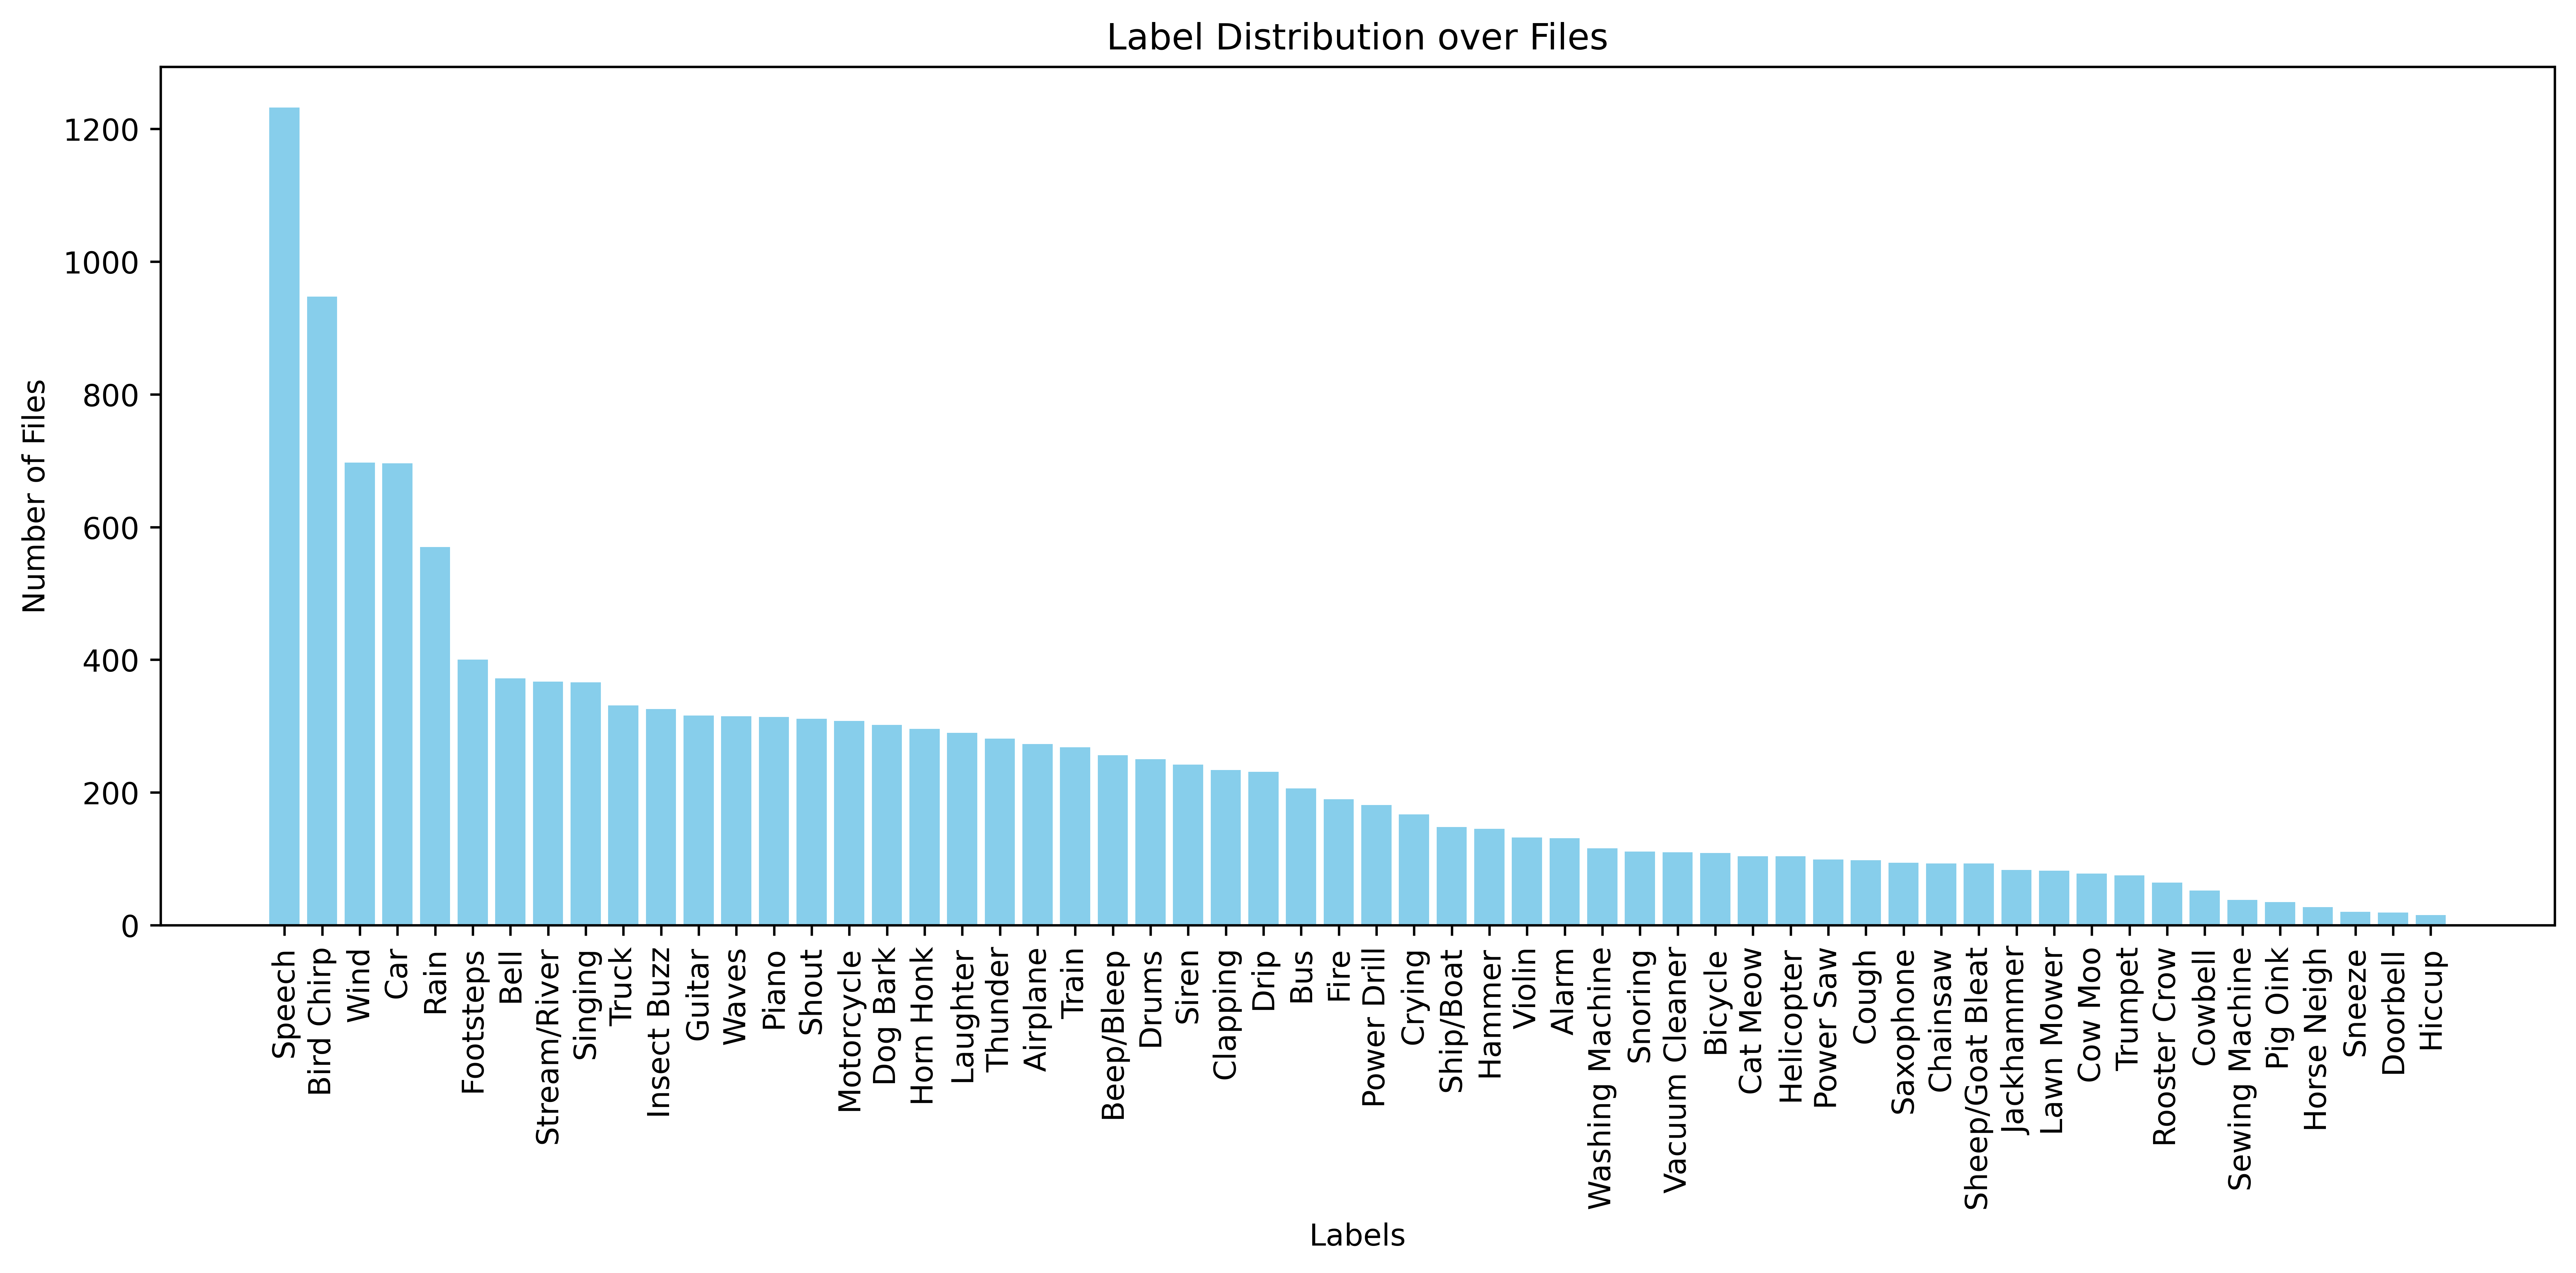
\includegraphics[width=\textwidth]{figs/2_Label Distribution over Files.png}
  \end{subfigure}
  \hfill
  \begin{subfigure}[b]{0.49\textwidth}
    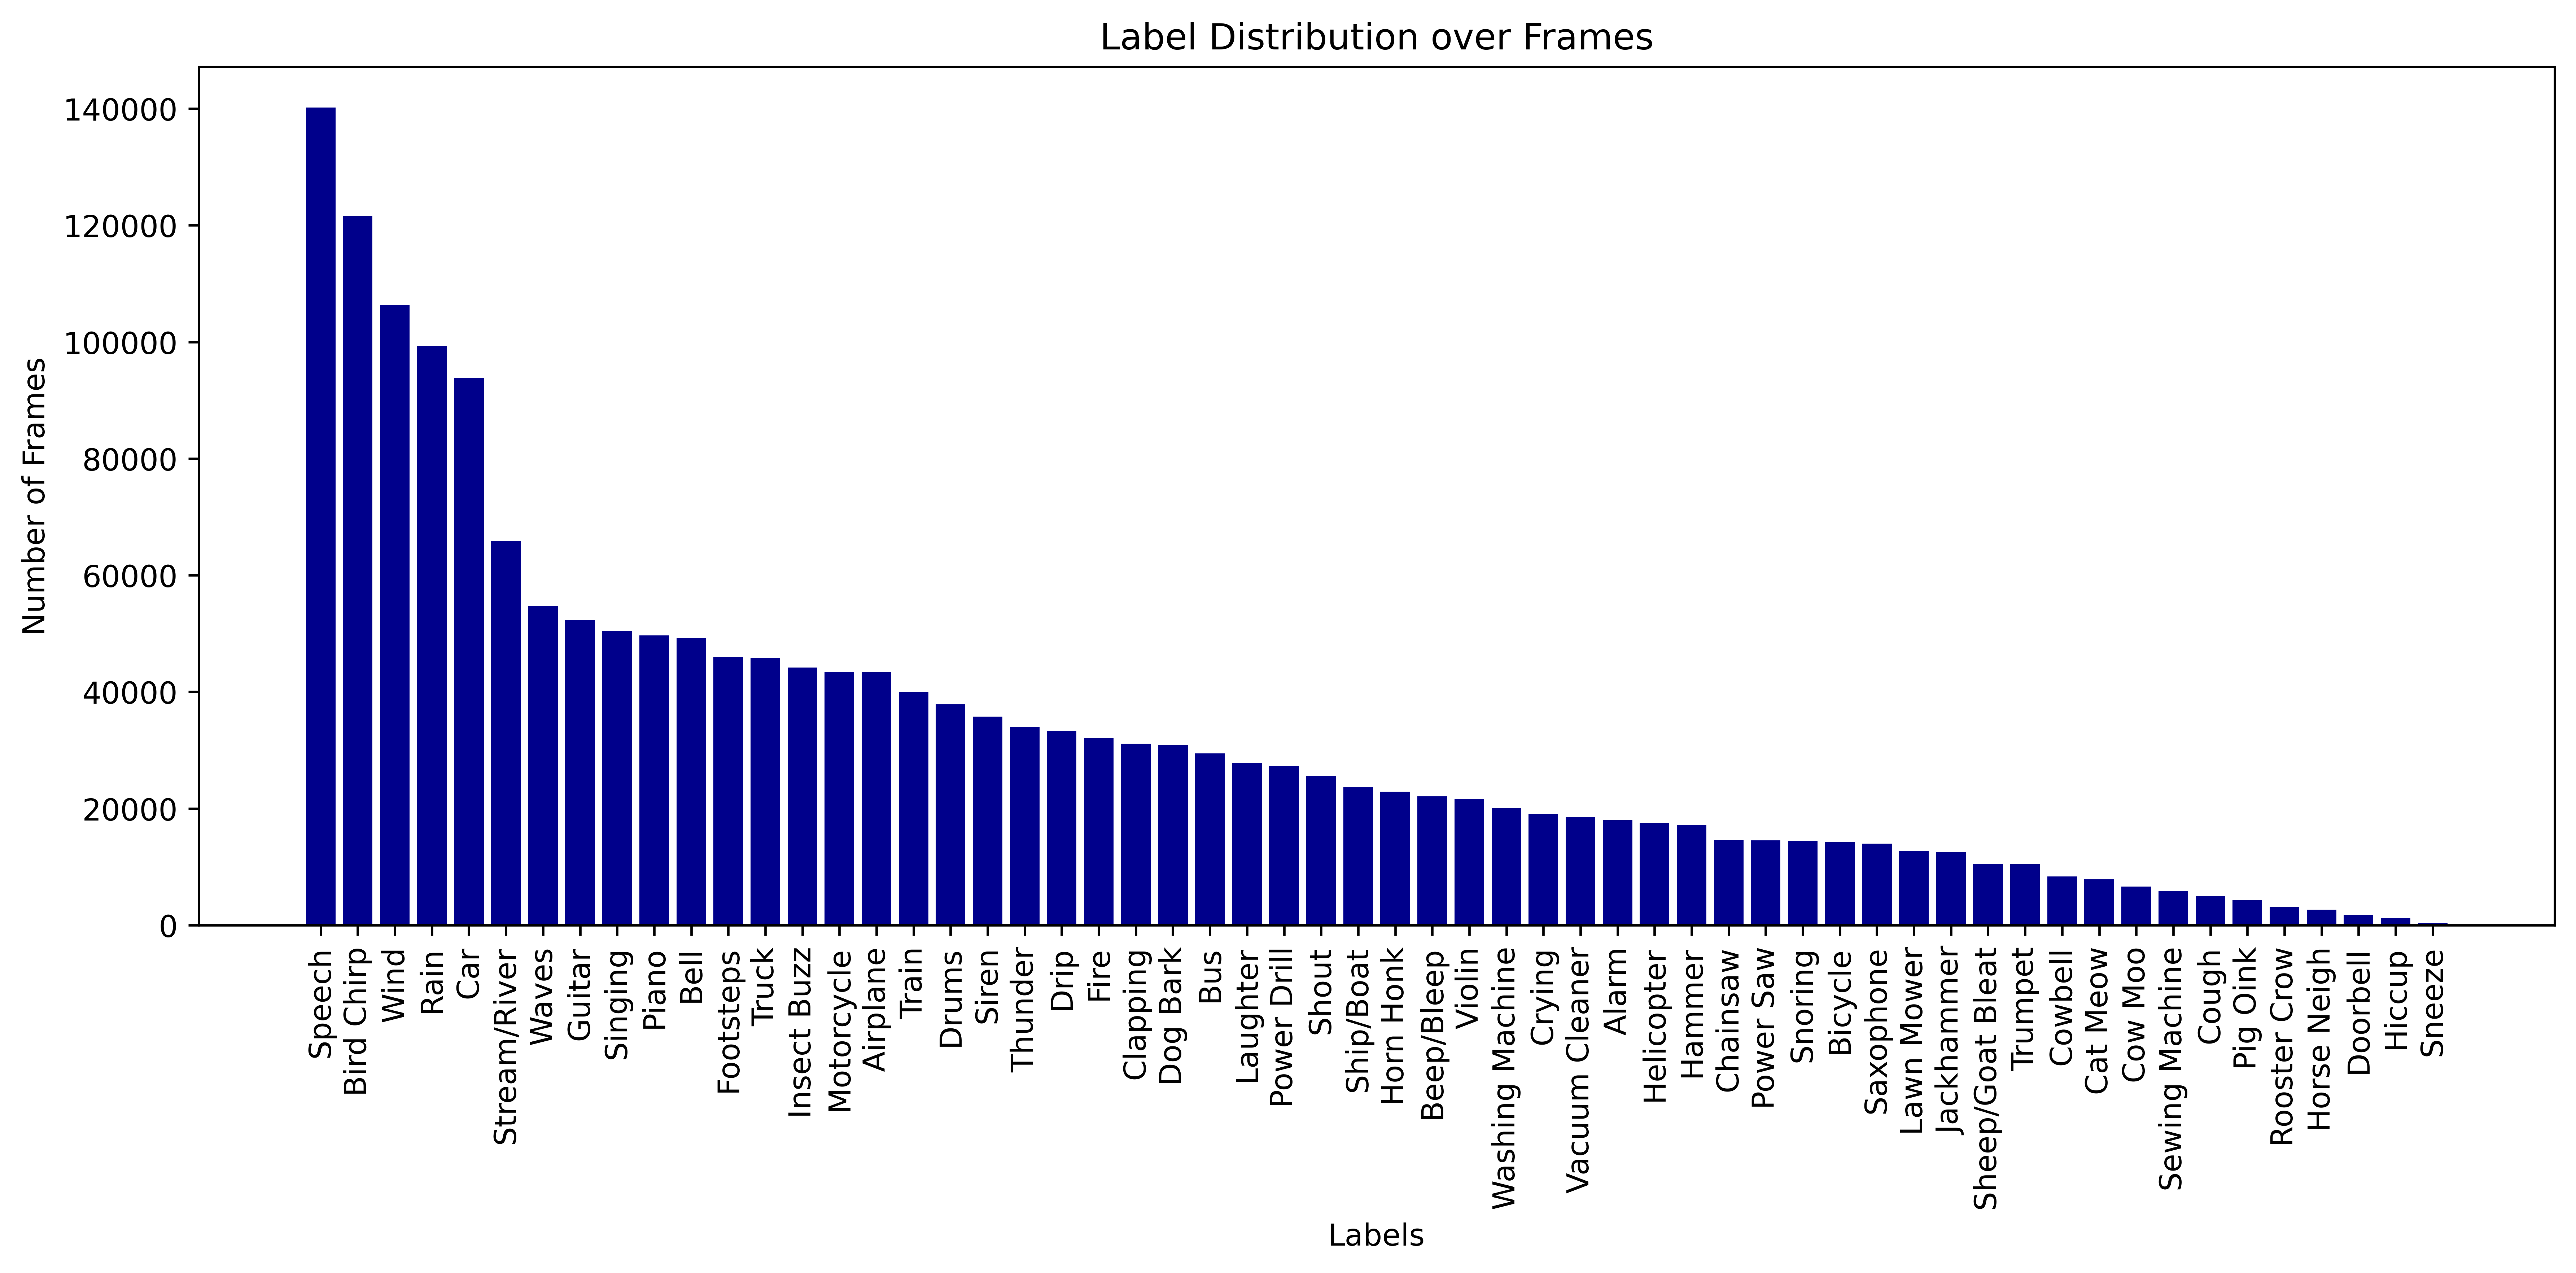
\includegraphics[width=\textwidth]{figs/2_Label Distribution over Frames.png}
  \end{subfigure}
  \caption{Label distribution}
  \label{fig:data-split}
\end{figure}



\subsection{Describe how you split the data for model selection and performance evaluation. }
\label{sec:Data Split:a}
To ensure a robust raining and proper model evaluation the available data set was independently split into three separate sets: Taring Set, Validation Set and Test set.


\begin{enumerate}
	\item {\bf Training Set: } The Training Set was used to train our classifiers. Training Set size was 60\% of our total data.
	
	\item {\bf Validation Set: } The Validation Set was used to estimate the performance of our model during training and to adust hyperparameter, while helping us to detect potential overfitting. Validation Set size was 20\% of our total data.

	\item {\bf Test Set: } The Test Set was used to evaluate the performance of our final model and estimate how well it would perform on unseen data. This Set was unseen by our classifiers prior to the final evaluation. Test Set size was 20\% of our total data.


    
\end{enumerate}

Using Cross-Validation was considered but ultimately not used as the provided data-set was large enough to have a low risk if underfitting and produced an overall satisfying results without the implementation of Cross-Validation.


We first loaded all the audio data with the features and the labels and split it into individual frames. 


\newpage

\subsection{Are there any potential factors that could cause information leakage across the data splits if they are not carefully designed? If yes, how did you address these risks?}

Yes, there are {\bf critical risks of information leakage} in audio classification if splits are not carefully designed:


\label{sec:Data Split:b}

\begin{itemize}
	\item {\bf Common Sources of Leakage: } 
    
		{\bf Temporal close audio segments: } If data is split by audio segments and not by full audio recording/session, temporal close audio segment can end up in different data sets. Because these segments will be closely related or even almost identical this would introduce data leakage to the data splits. 
        
		{\bf Same recording conditions: } If the same noise/audio source appears in both training and test sets, the model may learn source-specific features rather than class-specific ones. This can occur data from the same recording ends up in different data-sets. 

        {\bf Improper data splitting: } If data splitting is not done carefully, duplicates of the same sample might be included in multiple Sets causing data leakage.
        
        {\bf Leakage though data augmentation: } If data augmentation is applied before the data split and thus based on the entire dataset, this can result if information from the Test Set being included in the Training Set, causing leakage.\\
	
	\item {\bf Mitigation Strategies: } 
    
		{\bf File Splits:} We split the data not over the audio segments but over the full audio files. This ensures that temporally close segments and segments with the same recording condition are grouped into the same data set.

		{\bf Datasplit checking:} All data samples were indexed prior to data split and checked afterwards to ensure uniqueness among the samples. 
        
		{\bf Careful Preprocessing:} We avoided any preprocessing (e.g. feature normalization) that used statistics from the full dataset — we used only training data statistics. 
\end{itemize}


To avoid possible problems when splitting into the three data sets, 
we only split at file boundaries and tried to have an approximately equal distribution in all parts (stratification)  (\hyperref[fig:data-split]{Figure~\ref*{fig:data-split}}).
We worked in frames during pre-processing (normalization).




\subsection{Describe how you obtained unbiased final performance estimates for your models. }
\label{sec:Data Split:c}

Two main aspect were considered during model development to ensure a unbiased final performance estimation:

\begin{enumerate}
	
	\item {\bf Leakage minimization: } The prior mentioned data leakage techniques were carefully implemented to ensure a clear separation between the individual data-sets. 
    
	\item {\bf Strict Test Set Separation: } The test set was never used during training or validation. Final model evaluation was performed only once on the Test Set after all model development was completed.

%		If cross-validation is used, it’s done within the training+validation data.
%	
%	\item {\bf Repeated Experiments: } If randomness (e.g. in weight initialization or data sampling) affects results, the experiment is repeated with different seeds and the average + standard deviation is reported.
%
%	\item {\bf Stratified Sampling: } Ensures that the class distribution in all sets reflects that of the full dataset, which is particularly important in our case (unbalanced data sets).
\end{enumerate}





%\newpage


\section{Audio Features}
\label{sec:Audio Features}



\subsection{Which subset of audio features did you select for your final classifier? Describe the selection process and the criteria you used to make your choice.}
\label{sec:Audio Features:a}

After reflecting on the results from section \hyperref[sec:Labeling Function:b]{1.), b.)}, we have decided to run our experiments on the 'embeddings' feature as well as the other three features mentioned in that section. Even though the results imply heavy correlations and possible redundancies to the other three features - especially considering the possible creation process of these audio embeddings -  this still offered a slight increase in performance for tests we ran on a small scale. Performing all tests again using only the 'embeddings' feature would be computationally unfeasible, so we decided to play it safe.

Unfortunately we were not able to include context frames in our experiments as we did earlier, since the computational complexity was already extremely high and this would only have exaggerated the problem.


\subsection{Did you apply any preprocessing to the audio features? If so, explain which techniques you used and why they were necessary.}
\label{sec:Audio Features:b}

Preprocessing is an important step for ensuring consistency in the data and making the lives of models like Support-Vector-Machines much easier. We mainly normalized the data in order to to bring every example to a similar scale magnitude-wise, which generally improves performance and convergence rates.

We tried normalizing the data globally using the global mean and standard deviation from only our training set (to avoid data leakage), normalizing the features frame-wise to have unit mean and variance as well as a combination of these. In the end, doing only the latter proved to be the most performant, so that is what we did.





%\newpage


\section{Evaluation}
\label{sec:Evaluation}






\subsection{Which evaluation criterion did you choose to compare hyperparameter settings and algorithms, and why? }
\label{sec:Evaluation:a}

In terms of performance metrics we decided to record - per class label - both the Balanced Accuracy as well as the F1-score of our models predictions. As single measures of performance of a model, we then used the macro-averaged Balanced Accuracy / F1-score (over the 58 class labels), like was shown in the tutorial session. 

Balanced Accuracy, defined as the average recall per class (always binary in our case) obviously gives a more balanced performance metric, focusing on both the positive and negative classes. This metric was mainly included in order to be able to be able to compare the models to the baseline perfomance (see section \hyperref[sec:Evaluation:b]{4.), b.)}).\\
The F1-score on the other hand is most likely a much better suited performance metric for this task. Representing the harmonic mean of precision and recall, it has a stronger focus on predictions of the positive class. This makes sense for our task, as one classifier essentially consists of 58 binary classifiers - one per class label - which needs to predict in which frames it is present, i.e. positive. Generally this metric will be much lower than the Balanced Accuracy.


\subsection{What is the baseline performance? What could be the best possible performance? }
\label{sec:Evaluation:b}

In our case, the simple Majority-Class baseline classifier would always and for every label predict the negative class, since no single class-label is active in more than half of the frames in our dataset. This in turn would lead to a F1-score of 0 (since there are no True Positives). As already mentioned, in order to still be able to compare our models to the baseline we also recorded the Balanced Accuracy. Obviously, as the recall for the negative class would be 1 and for the positive class 0, our baseline Balanced Accuracy is 0.5.

Considering the unavoidable noise, inaccuracies and mislabelings in the data, we suspect the best possible performance one could ever achieve to be around an F1-score of 0.9 up to 0.95.




%\newpage


\section{Experiments}
\label{sec:Experiments}






\subsection{For at least three different classifiers, systematically vary the most important hyperparameters and answer the following questions for each of them: }
\label{sec:Experiments:a}



\subsubsection{How does classification performance change with varying hyperparameter values? Visualize the change in performance. }
\label{sec:Experiments:a-1}



\subsubsection{(To what extent) Does overfitting or underfitting occur, and what does it depend on? }
\label{sec:Experiments:a-2}






\subsection{After selecting appropriate hyperparameters, compare the final performance estimate of the three classifiers. }
\label{sec:Experiments:b}




%\newpage


\section{Analysing Predictions}
\label{sec:Analysing Predictions}



Find two interesting audio files that have not been used for training and qualitatively evaluate your classifier’s predictions. 



\subsection{Use the spectrogram and the sequence of predictions to visualize the classifier output. }
\label{sec:Analysing Predictions:a}






\subsection{Listen to the audios and inspect the corresponding predictions of the classifier. }
\label{sec:Analysing Predictions:b}



\subsubsection{How well does the classifier recognize the classes? }
\label{sec:Analysing Predictions:b-1}






\subsection{What are particular problematic conditions that cause the classifier to mispredict classes? }
\label{sec:Analysing Predictions:c}



\subsubsection{Can you think of simple postprocessing steps that might help improve the predictions? }
\label{sec:Experiments:c-1}





\end{document}



